% Chapter 1

\chapter{Introducción General} % Main chapter title

\label{Chapter1} % For referencing the chapter elsewhere, use \ref{Chapter1} 
\label{IntroGeneral}

%----------------------------------------------------------------------------------------

% Define some commands to keep the formatting separated from the content 
\newcommand{\keyword}[1]{\textbf{#1}}
\newcommand{\tabhead}[1]{\textbf{#1}}
\newcommand{\code}[1]{\texttt{#1}}
\newcommand{\file}[1]{\texttt{\bfseries#1}}
\newcommand{\option}[1]{\texttt{\itshape#1}}
\newcommand{\grados}{$^{\circ}$}

%----------------------------------------------------------------------------------------
La idea de este capítulo consiste en presentar la motivación que impulsó el desarrollo del equipo, así como también mostrar una breve reseña de algunas soluciones ya disponibles comercialmente.

\section{Motivación}

El proyecto surgió de la necesidad de desarrollar un producto que no solo permitiera automatizar el encendido y apagado de una carga eléctrica, sino que también brindara información acerca del consumo de la misma.

%TODO: agregar referencia de domótica.
En los últimos años, uno de los principales intereses de los consumidores a nivel mundial es el de la domótica [referencia], entendiéndose por esta al conjunto de sistemas y equipos que permiten automatizar una casa, abarcando la seguridad, el confort y la gestión energética. Es en este último aspecto en el cual se encuadra el presente proyecto.

Uno de las funcionalidades más básicas que se pretende esté presente en un sistema de domótica consiste en el control de un aparato eléctrico. Esto incluye tanto el encendido y apagado del mismo como la posibilidad de poder programar horarios específicos de funcionamiento.

Sumado al mero deseo de poder controlar un dispositivo eléctrico de forma sencilla, se encuentra el hecho de que los usuarios tienen una mayor consciencia acerca de la importancia de tener un consumo eléctrico responsable. En nuestro país uno de los principales impulsores de esta concientización son los crecientes costos asociados a la energía eléctrica.

En los últimos meses, la cuestión del costo del servicio eléctrico ha sido uno de los principales temas de debate. En la Figura \ref{fig:costo_caba} puede verse la evolución del costo del kWh (kilowatt hora) en la Ciudad Autónoma de Buenos Aires, desde el año 1993 hasta el presente.

\begin{figure}[h]
	\centering
	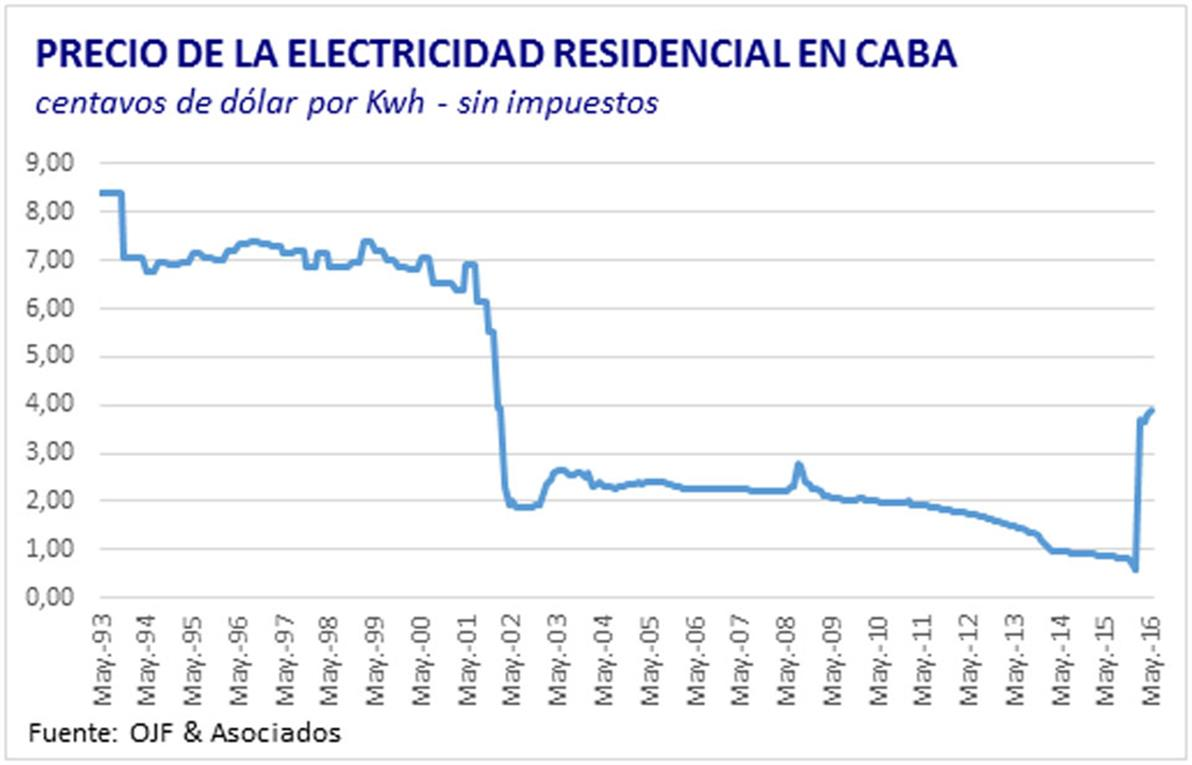
\includegraphics[width=12cm]{./Figures/1_1_costo_electricidad_caba.png}
	\caption{Evolución del costo de la energía eléctrica en la Ciudad Autónoma de Buenos Aires.}
	\label{fig:costo_caba}
\end{figure}

La preocupación de los consumidores se ve justificada en el hecho de que durante los primeros meses del año 2016 se produjo el primer aumento brusco en la tarifa, hecho que no ocurría desde hacía más de diez años. Y es en este contexto que se consideró importante desarrollar un producto que le permita al usuario conocer de una forma práctica y fácil la información del consumo de los aparatos eléctricos que utiliza cotidianamente. 

Y es importante destacar, que en la mayoría de los casos, la única información que posee el consumidor acerca de su consumo es la cantidad de energía consumida en un mes o en un bimestre por toda su instalación eléctrica. Contando con este único dato, es difícil poder tomar decisiones que modifican la forma de consumir energía eléctrica de las personas. El equipo propuesto en este trabajo buscó ofrecer una mayor información de cada dispositivo eléctrico al que se lo conecte. De esta forma, el usuario puede conocer en tiempo real las características del consumo de un aparato eléctrico.

Contando con información más detallada, el usuario:
\begin{itemize}
\item Identificar consumos de energía desconocidos.
\item Ajustar los horarios de funcionamiento del aparato eléctrico, adecuándolos a los momentos del día en el que realmente son necesarios.
\item Estimar el costo de  la energía consumida por cada aparato eléctrico.
\end{itemize}

Otro impulsor del proyecto fue que la disponibilidad local de equipos de automatización con estas características es extremadamente baja. Las soluciones que se comentan en la Sección \ref{section:soluciones_comerciales} pueden ser compradas a través de Internet, pero no de una forma sencilla en los comercios nacionales. Esta situación hace propicio el ofrecer una alternativa de fabricación nacional que pueda ser adquirida junto con otros productos que conformen una solución más completa de domótica.



\section{Soluciones comerciales existentes}
\label{section:soluciones_comerciales}

Actualmente, varias empresas a nivel mundial ofrecen productos para la automatización de cargas eléctricas. Comúnmente se denomina a estos equipos Smart Plugs y consisten básicamente en un equipo que se conecta al tomacorriente y al cual se conecta el aparato eléctrico que se quiere controlar. De esta forma, el Smart Plug queda conectado entre el tomacorriente y la carga eléctrica y permite:

\begin{itemize}
\item Encender y apagar la carga.
\item Conocer los parámetros eléctricos de la carga: tensión, corriente, factor de potencia, potencia activa, etc.
\item Informar la energía consumida por el aparato.
\item Programar horarios de encendido y apagado.
\item Monitorear la temperatura del equipo.
\end{itemize}

No todos los equipos comerciales cumplen con todas estas funcionalidades simultáneamente . Sin embargo, un punto común a todos los Smart Plugs comerciales es que ofrecen algún tipo de aplicación móvil para poder gestionar los Plugs dentro de una casa. Este aspecto es uno de los más importante en el diseño de un producto de estas características ya que la información que proveen los Smart Plugs debe ser mostrada al usuario de forma sencilla y útil para que pueda ser aprovechada.

Otra característica común es que muchos de los equipo son fabricados por empresas dedicadas a comercializar productos para redes de computadoras. De esta forma, se tienen algunos ejemplos como WeMo de la empresa Belkin, DS-W215 de D-Link y HS110 de TP-Link. En esta sección se describirán brevemente estos dos últimos equipos>

\begin{itemize}
\item \textbf{D-Link - DSP-W21}. Este dispositivo desarrollado por D-Link puede verse en la Figura \ref{fig:smartplug_dlink}. Las principales funciones que ofrece son: encendido/apagado de la carga tanto a través de la aplicación móvil como de un interruptor en el propio equipo, conexión a la red WiFi a través de WPS \footnote{WiFi Protected Setup. Es un conjunto de mecanismos que buscan facilitar la incorporación de un equipo a una red WiFi. Generalmente, para iniciar el proceso de WPS se debe presionar un botón en el producto que se desea incorporar a la red y se debe presionar el botón de WPS en el router WiFi. Una vez hecho esto el dispositivo se incorporará a la red.}, programación horaria del encendido/apagado y registro del consumo.

\begin{figure}[h]
	\centering
	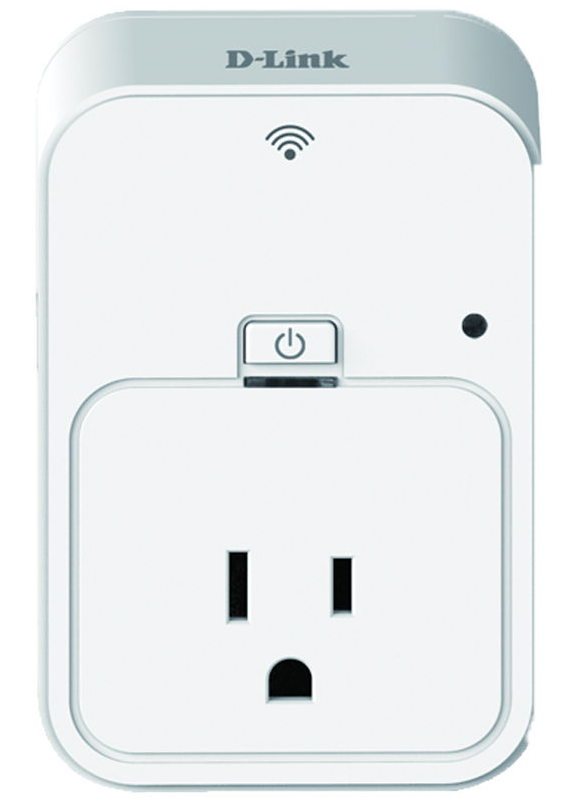
\includegraphics[width=6cm]{./Figures/1_2_DSP-W215.png}
	\caption{Smart Plug DSP-W215 de la empresa D-LINK}
	\label{fig:smartplug_dlink}
\end{figure}

La aplicación (disponible para dispositivos con sistema operativo Android y iOS) le permite al usuario controlar la carga desde la misma red WiFi en la que se encuentran los Smart Plugs y desde la red móvil. Esta aplicación también permite controlor otros productos de la línea  \textit{mydlink} como pueden ser cámaras y detectores de movimiento.

A diferencia de otros Smart Plugs, el gabinete es considerablemente grande (96 x 62 x 45 mm) lo cual es resaltado como un punto negativo en las reseñas de este producto.

Al momento de escribir esta memoria, el precio de este producto era de 50 dólares en Estados Unidos y no estaba disponible para ser adquirido en los comercios argentinos. Además, entre los tipos de enchufes disponibles para conectar la carga no se encuentra disponible el usado en Argentina.

\item \textbf{TP-Link - HS110}. Al igual que el anterior Smart Plug, el HS110 permite controlar una carga desde una aplicación móvil (disponible en Android y en iOS), pudiendo visualizar el tiempo total de encendido del dispositivo y la energía consumida tanto actual como en las semanas previas. Este producto ofrece un gabinete más reducido que el Smart Plug de D-Link. Puede verse una imagen del mismo en la Figura \ref{fig:smartplug_tplink}.

\begin{figure}[h]
	\centering
	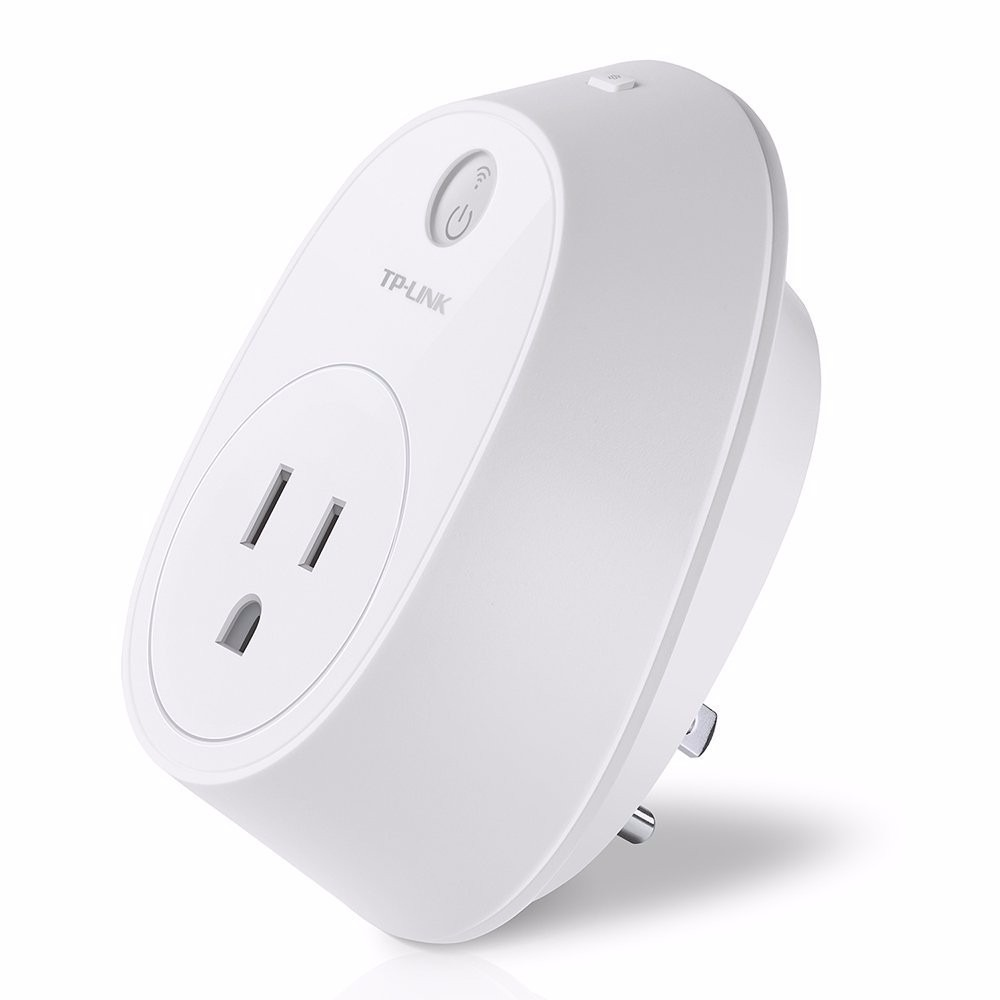
\includegraphics[width=6cm]{./Figures/1_2_TP-LINK-HS110.png}
	\caption{Smart Plug HS110 de la empresa TP-LINK}
	\label{fig:smartplug_tplink}
\end{figure}

Como diferencias con el producto de D-Link, se pueden mencionar que cada Smart Plug puede ser configurado para que se encienda y se apague de forma aleatoria para simular la presencia de una persona en el hogar.También es compatible con Amazon Echo, un producto que permite controlar dispositivos mediante comandos de voz.

El precio en Estados Unidos es cercano a los 40 dólares y al igual que el Smart Plug de D-Link no es vendido localmente.

\end{itemize}


\section{Objetivos}





%----------------------------------------------------------------------------------------






